% Level ceiling (grade 8): powers of ten written in math mode as
% $3 \times 10^8$ (math g8-03); NO \qty e-notation and no formal
% scientific-notation machinery (both arrive in grade 9).
\chapter{光速；宇宙中的距离}\label{ch:g8:speed-of-light}

七年来，本书一直暗示光“几乎等同于瞬时”——
闪电之前的那道闪光，看见的击打即刻启动秒表。
本章兑现本书最古老的承诺：光速并非无限，
人类竟在种种困难之下测出了它；
这个数字如此巨大，以至于同时成为
天文学的尺子，也是天文学的时光机。

\section{不可能完成的测量}

\begin{example}[两座山上的灯笼]\label{ex:g8:speed-of-light:galileo}
四百年前，伟大的实验先驱让两位观测者
夜间站在远处的两座山上，各持一盏带快门的灯笼：
一方看见对方的灯光后便打开自己的灯，往返延迟本应揭示光速。
他们测得的延迟，其实只是人的反应时间；两山之间，
光真正穿越的时间只需
\emph{百万分之几}秒。
实验失败得十分壮观——至少证明了，光
比山顶上任何计时器能测出的都要快，并促使
天文学家去寻找更长的“赛道”。
\end{example}

\begin{example}[迟到的月亮]\label{ex:g8:speed-of-light:romer}
这条“赛道”由木星提供。它最内侧的一颗大卫星
以极其规律的周期进入木星的阴影——
这是天上的一座时钟。然而，一位耐心的天文学家
发现在那些月份里，这座钟\emph{晚点}了好几分钟——
地球轨道已把我们带到太阳远离木星的一侧，
而当我们再度靠近时，它又提前了。
他的推断是：月亮是准时的——它的\emph{光}
被延迟了，需要额外的时间穿越
地球轨道多出的宽度。由这份迟到与轨道的大小，
得出了光速的第一个估计——以十七世纪的水准而言，
它惊人地接近真实值。
\end{example}

\begin{omfigure}
\begin{tikzpicture}[scale=0.8]
  \fill[omThm] (4.6,1.7) circle (0.42);
  \node[below, font=\small] at (4.6,1.1) {太阳};
  \draw[dashed, omExo] (4.6,1.7) ellipse (2.6 and 1.05);
  \fill[omDef] (2.0,1.7) circle (0.18);
  \node[below, font=\footnotesize] at (2.0,1.3) {地球（近）};
  \fill[omDef, opacity=0.5] (7.2,1.7) circle (0.18);
  \node[below, font=\footnotesize] at (7.5,1.3) {地球（远）};
  \fill[omExo] (0.6,1.7) circle (0.3);
  \node[above, font=\small] at (0.6,2.1) {木星及其卫星};
  \draw[-Stealth, omThm, thick] (0.95,1.78) -- (1.8,1.74);
  \draw[-Stealth, omThm, thick] (0.95,1.62) -- (7.0,1.64);
  \node[below, font=\footnotesize, omThm] at (5.2,0.35)
    {远处位置的光需多穿越整条轨道};
\end{tikzpicture}

{\small 迟到的月亮：来自木星的食讯
传到位于远侧的地球，比预定时间晚了好几分钟——
这延迟便是光赶路所耗的时间。}
\end{omfigure}

\begin{proposition}[光速]\label{prop:g8:speed-of-light:value}
在真空中——在空气中近似亦然——光
传播速度为
\[
c = \qty{300000}{km/s} = 3 \times 10^{8}\ \unit{m/s},
\]
每秒三十万千米：两次心跳之间，
光可绕地球七圈半。混合光中的每种颜色，
在真空中都以同样的 $c$ 传播；
任何携带物质或消息的东西，从未被测得比它更快。此后，
地面上的巧思证实了天文学家的结论——一束光
被旋转的带齿圆盘切断，奔向八千米外的镜子，
再穿过下一个齿隙返回，而
现代仪器已将 $c$ 测得确凿无疑，以至于
米本身如今就由它来定义。
\end{proposition}

\begin{example}[近邻天体的旅行时间]\label{ex:g8:speed-of-light:times}
由 $t = d/c$，太阳系便有了一张时刻表。其中
月球距离 \qty{384000}{km}：$384000 \div 300000 \approx
\qty{1.3}{s}$——地月无线电通话总带着那段
尴尬的停顿。太阳距离 $150$ 百万千米：$150000000 \div
300000 = \qty{500}{s}$——八分二十秒：阳光总是
八分钟前的新闻。火星典型距离为 $2 \times
10^{8}$ 千米，约十一分钟——巡视车驾驶员发出当天的
计划后只能等待；任何操纵杆都无法在
长达二十分钟的往返延迟下实时操控。
\end{example}

\begin{omfigure}
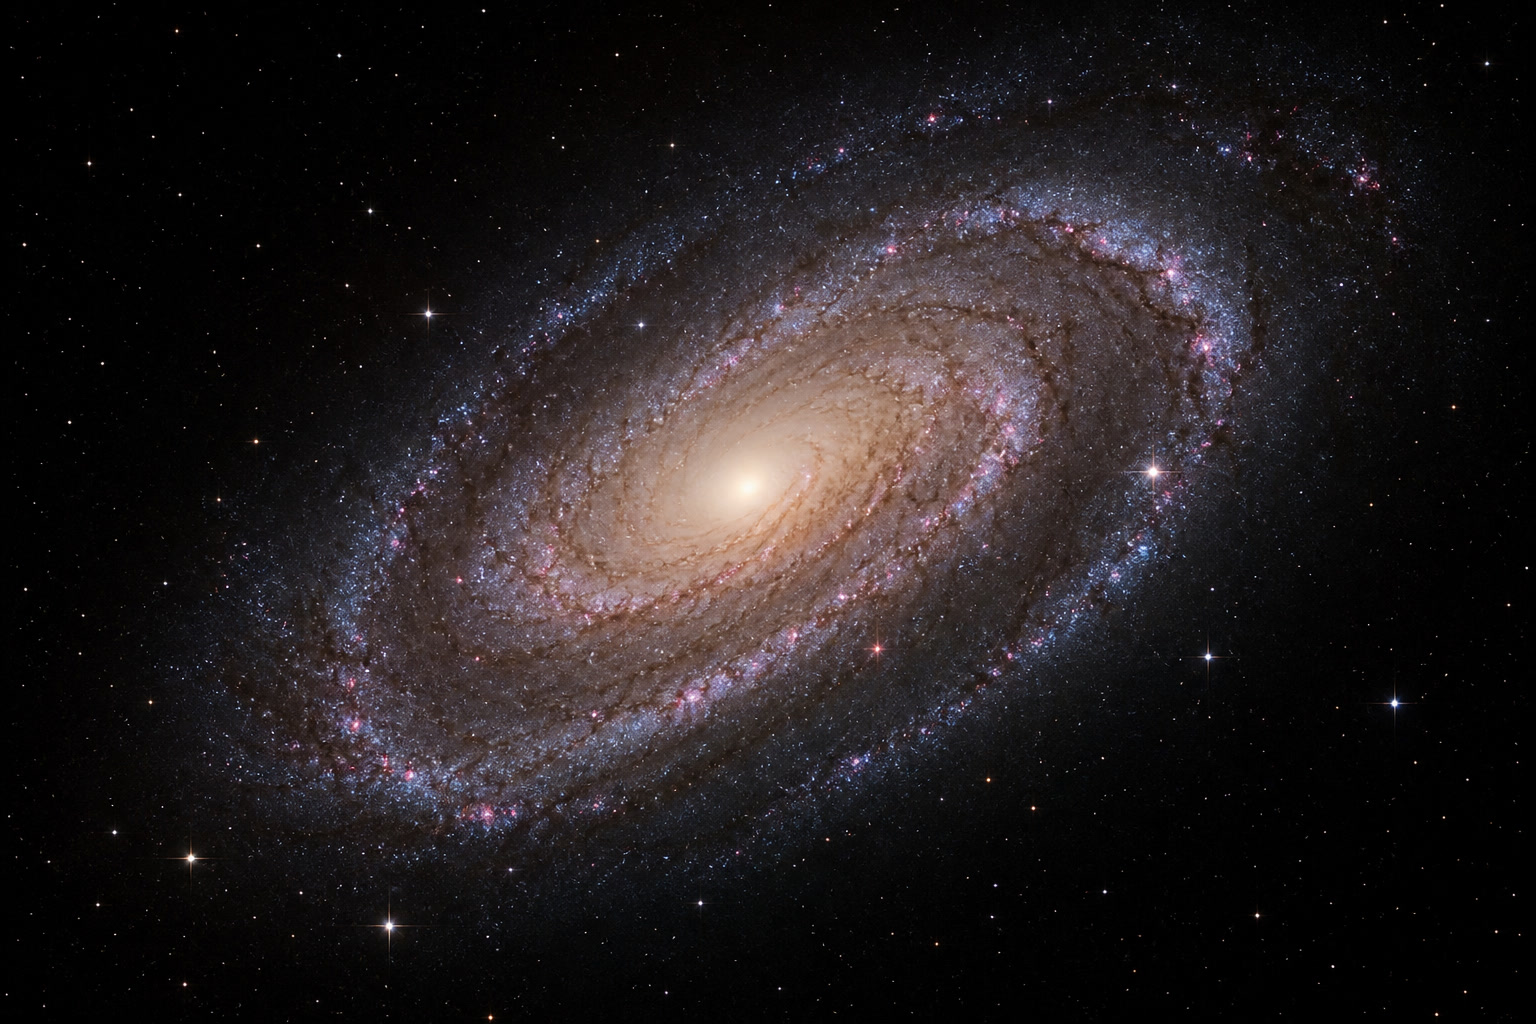
\includegraphics[width=0.55\linewidth]{images/book1/ai/g8-universe-galaxy.jpg}

{\small 一个旋涡星系：其恒星发出的光，在抵达任何望远镜之前，要穿越数百万年的空旷太空。}
\end{omfigure}

\section{光年}

\begin{definition}[光年]\label{def:g8:speed-of-light:lightyear}
称\emph{光年}\index{光年}为\emph{距离}：
即光在一年中所走过的路程——约 $9.5 \times
10^{12}$ 千米，接近十万亿千米。这个名称
容易误导急躁的人（它不是时间，正如
“脚步”并不是“脚”一样）；天文学家之所以使用它，是因为
千米在天空的真实尺度面前显得太小。
\end{definition}

\begin{example}[近邻的光年尺度]\label{ex:g8:speed-of-light:ladder}
太阳之外最近的恒星：约 $4$ 光年——
今晚的光子离开它时，你还在读物理的
最初几章。冬季夜空中的亮星：数十
至数百光年。银河，我们所在的恒星之城，
直径约 $100000$ 光年。最近的大型邻居星系
约 $2.5$ 百万光年——它
那一抹微弱的光斑，在暗适应后的裸眼中可见，是
人类不借助仪器所能看到的最古老的光。
\end{example}

\begin{proposition}[望远镜是时光机器]\label{prop:g8:speed-of-light:timemachine}
因为光传来的“消息”以 $c$ 的速度传播，而宇宙极其浩瀚，
\emph{看得远，就是回望过去}。距离 $4$
光年的恒星，呈现的是它 $4$ 年前的模样；
邻近的星系，呈现的是我们的祖先第一次打制
石器时的模样。g5 观星者的怀疑，如今已是一条
算术定理：凡朝外对准的望远镜，都朝向过去，
天文学便是借星光阅读的历史。
\end{proposition}

\begin{method}[距离与回溯时间的换算]\label{met:g8:speed-of-light:convert}
\begin{enumerate}
  \item 以光年为单位的距离 $\to$ 以年为单位的回溯时间：两者
        数值相同——这正是该单位的妙处；
  \item 以千米为单位的距离 $\to$ 光行时间：先除以
        \qty{300000}{km/s}，再把秒换算成
        分钟、小时或年；
  \item 光年 $\to$ 千米（很少值得这样做）：
        乘以 $9.5 \times 10^{12}$——并记住
        天文学家为何很少这样做。
\end{enumerate}
\end{method}

\begin{remark}[远方的“现在”意味着什么]\label{rem:g8:speed-of-light:now}
四光年外的那颗恒星，是否仍在\emph{此刻}发光？
几乎可以肯定——恒星寿命很长——但没有任何
比光本身更快的消息能够传到我们这里：最新的可能消息
也已过时四年，始终如此。对于深空，问题
变得更加奇异：大型望远镜中一些最暗淡的光斑，
是那些光在地球存在之前就已发出的星系。
物理学会在大学阶段进一步厘清“远处的现在”
究竟意味着什么；眼下这一年，请带着诚实的版本：
天空不是一幅景象——
它是一座档案馆。
\end{remark}

\section{练习}

\begin{exercise}[$\star$]\label{exo:g8:speed-of-light:1}
求 $c$，分别以 \unit{km/s} 和 \unit{m/s} 为单位（用 10 的幂
形式表示）。两座山上的尝试哪里失败了？为什么？
\end{exercise}

\begin{exercise}[$\star$]\label{exo:g8:speed-of-light:2}
用三句话复述“月亮迟到”的论证：什么是准时的，
什么是迟到的，以及这段迟到测量了什么。
\end{exercise}

\begin{exercise}[$\star$]\label{exo:g8:speed-of-light:3}
计算光的传播时间：月球（\qty{384000}{km}）；太阳
（$150$ 百万千米）。为什么阳光是“旧闻”？
\end{exercise}

\begin{exercise}[$\star$]\label{exo:g8:speed-of-light:4}
光年是时间还是距离？请给出它的定义，并给出它
以千米为单位的大小（用 10 的幂形式表示）。
\end{exercise}

\begin{exercise}[$\star$]\label{exo:g8:speed-of-light:5}
最近的恒星约位于 $4$ 光年之外。今晚的
回溯时间是多少？当它的光离开时，
你正在做什么？
\end{exercise}

\begin{exercise}[$\star$]\label{exo:g8:speed-of-light:6}
为什么无法在地球上用操纵杆遥控火星车？请用
时间表例子中的数据。
\end{exercise}

\begin{exercise}[$\star$]\label{exo:g8:speed-of-light:7}
按回溯时间排序：月球；太阳；最近的恒星；
近邻星系——并给出各自的大致数值。
\end{exercise}

\begin{exercise}[$\star$]\label{exo:g8:speed-of-light:8}
“米现在是由 $c$ 定义的。”这句话说明，
在尺子与光之间，物理学家更深信不疑的是
哪一个？
\end{exercise}

\begin{exercise}[$\star\star$]\label{exo:g8:speed-of-light:9}
雷达测距：一个以 $c$ 传播的无线电脉冲，经月球反射
后约 \qty{2.6}{s} 返回。由这次往返的时间求出月球的
距离，并说出可以沿用过来的一条旧声呐规律的
名称。
\end{exercise}

\begin{exercise}[$\star\star$]\label{exo:g8:speed-of-light:10}
按档案的深度排序：你房间里台灯发出的光
（\qty{3}{m}）；太阳；距离 $100$ 光年的恒星；
近邻星系。对于台灯，估算以十亿分之一秒计的
回溯时间（$3 \div (3 \times 10^{8})$——
用文字把它说清楚）。
\end{exercise}

\begin{exercise}[$\star\star$]\label{exo:g8:speed-of-light:11}
一则新闻报道说：“天文学家上周二观测到一颗恒星
爆炸，距离 $8000$ 光年。”请用诚实的时态改写
这句话，说明爆炸是何时发生的，
以及上周二究竟发生了什么？
\end{exercise}

\begin{exercise}[$\star\star\star$]\label{exo:g8:speed-of-light:12}
“月亮迟到”的迟到量在约 $1000$ 秒时达到峰值——
这是光穿越地球轨道整个宽度所需的时间，
约 $3 \times 10^{8}$ 千米。请亲自做一遍十七世纪的
除法运算，并与现代的 $c$ 比较：
天空最初给出的答案有多诚实？
\end{exercise}

\section{问题：任务控制中心}

\begin{problem}[{周末问题 --- 深空
任务控制中心值班；从月球到恒星的光迟滞通话；
操作手册}]\label{pb:g8:speed-of-light:1}
今晚你负责通信台：每条消息
都以 $c = \qty{300000}{km/s}$ 传播，光的迟滞
决定着每一项决策。

\medskip\noindent\textbf{第一部分 --- 近距离操作。}
\begin{enumerate}
  \item 月球基地（\qty{384000}{km}）请求
        确认一次物资投放。你发出“已确认”之后，
        基地要过多久才能听到？最快多久能收到
        他们的回执？
  \item 一颗位于 \qty{36000}{km} 高轨道上的卫星转播
        一路电视信号。计算其单程迟滞——
        并说明为何经由此类卫星的洲际电话
        会有一丝可察觉的停顿
        （往返一次，上行加下行）。
  \item 太阳天文台报告一次强耀斑，称其“正在
        发生”。请纠正操作员的说法：这次耀斑
        究竟是何时爆发的？
  \item 规程要求所有时钟都要计入迟滞。哪一条
        近地链路——月球或高轨道卫星——需要
        更大的余量？两者大约相差多少倍？
\end{enumerate}

\medskip\noindent\textbf{第二部分 --- 火星窗口。}
今晚火星位于 $1.8 \times 10^{8}$ 千米处。
\begin{enumerate}[resume]
  \item 分别以秒和分钟计算单程迟滞。
  \item 巡视车遇到一道意外的裂缝，其
        摄像头显示它正以步行速度靠近。请说明，
        结合往返时间，为何用操纵杆遥控救援
        毫无希望——以及巡视车因此必须自带哪些
        设备。
  \item 当晚计划的上传需要 \qty{3}{min} 的
        传输时间，外加迟滞。上传须于何时开始，
        才能使巡视车在 21:00（控制中心时间）
        完整接收？
  \item 六个月后，火星将位于 $3.8 \times
        10^{8}$ 千米处。迟滞会如何变化？这对理解
        行星的“距离”一词有何启示？
\end{enumerate}

\medskip\noindent\textbf{第三部分 --- 远程台。}
\begin{enumerate}[resume]
  \item 一艘星际探测器已与地球相距整整一
        个光\emph{日}。请以千米表示该距离（用 10 的幂表示；
        一天为 $86400$ 秒），
        并求与该探测器往返通话的
        时间。
  \item 后排的幻想家起草了一份“给最近恒星的
        消息”。请改为拟定时间表：今晚发出，
        最早何时能收到任何回复？
  \item 档案墙上展示了今晚拍摄的邻近星系的深空图像，
        该星系距离 $2.5$ 百万光年。请补上图注
        应有的诚实时态——若有人身在那里观看，
        这张快照所传回的是地球
        过去的哪个时代？
  \item 交班记录：写下本台的三条规则——
        一条关于“瞬时”（即没有任何事是瞬时的），一条关于
        操纵杆与迟滞，一条关于望远镜与
        档案。
\end{enumerate}
\end{problem}
